\documentclass[10pt]{beamer}

%\usepackage[backend=bibtex,firstinits=true,style=verbose-inote,citestyle=authortitle]{biblatex}
\usepackage{bm}
\usepackage{graphicx}
\usepackage{subcaption}
\usepackage{amsmath}
\usepackage{makecell}
\usepackage{filecontents}
\usepackage[doi=false,isbn=false,url=false,eprint=false]{biblatex}
% \newcommand{\expect}[2][]{
\ifthenelse{\equal{#1}{}}{
\mathbb{E}\left[#2\right]
}{
\underset{#1}{\mathbb{E}}\left[#2\right]
}}

\newcommand{\cov}[2][]{
\ifthenelse{\equal{#1}{}}{
\text{Cov}\left[#2\right]
}{
\underset{#1}{\text{Cov}}\left[#2\right]
}}


\newcommand{\var}[2][]{
\ifthenelse{\equal{#1}{}}{
\text{Var}[#2]
}{
\underset{#1}{\text{Var}}[#2]
}}

\newcommand{\loss}[2][]{
\ifthenelse{\equal{#1}{}}{
\mathcal{L}(#2)
}{
\mathcal{L}_{#1}(#2)
}}

\newcommand{\kl}[2]{
\text{D}_\text{KL}[#1 \parallel #2]
}

\newcommand{\R}{\mathbb{R}}
%\newcommand{\Prob}{\mathbb{P}}

\newcommand{\1}[1]{\mathds{1}\{#1\}}


%\usecolortheme{dolphin}
\setbeamertemplate{navigation symbols}{}
\setbeamertemplate{section in toc}{\inserttocsectionnumber.~\inserttocsection}

\newcommand{\expect}[2][]{
\ifthenelse{\equal{#1}{}}{
\mathbb{E}\left[#2\right]
}{
\underset{#1}{\mathbb{E}}\left[#2\right]
}}

\begin{filecontents*}{references.bib}
@incollection{DGR,
title = {Continual Learning with Deep Generative Replay},
author = {Shin, Hanul and Lee, Jung Kwon and Kim, Jaehong and Kim, Jiwon},
booktitle = {Advances in Neural Information Processing Systems 30},
editor = {I. Guyon and U. V. Luxburg and S. Bengio and H. Wallach and R. Fergus and S. Vishwanathan and R. Garnett},
pages = {2990--2999},
year = {2017},
publisher = {Curran Associates, Inc.},
url = {http://papers.nips.cc/paper/6892-continual-learning-with-deep-generative-replay.pdf}
}
@incollection{MeRGAN,
title = {Memory Replay GANs: Learning to Generate New Categories without Forgetting},
author = {Wu, Chenshen and Herranz, Luis and Liu, Xialei and wang, yaxing and van de Weijer, Joost and Raducanu, Bogdan},
booktitle = {Advances in Neural Information Processing Systems 31},
pages = {5962--5972},
year = {2018},
publisher = {Curran Associates, Inc.},
url = {http://papers.nips.cc/paper/7836-memory-replay-gans-learning-to-generate-new-categories-without-forgetting.pdf}
}
@article{PathNet,
  author    = {Chrisantha Fernando and
               Dylan Banarse and
               Charles Blundell and
               Yori Zwols and
               David Ha and
               Andrei A. Rusu and
               Alexander Pritzel and
               Daan Wierstra},
  title     = {PathNet: Evolution Channels Gradient Descent in Super Neural Networks},
  journal   = {CoRR},
  volume    = {abs/1701.08734},
  year      = {2017},
  url       = {http://arxiv.org/abs/1701.08734},
  archivePrefix = {arXiv},
  eprint    = {1701.08734},
  timestamp = {Mon, 13 Aug 2018 16:49:06 +0200},
  biburl    = {https://dblp.org/rec/bib/journals/corr/FernandoBBZHRPW17},
  bibsource = {dblp computer science bibliography, https://dblp.org}
}
@article {EWC,
	author = {Kirkpatrick, James and Pascanu, Razvan and Rabinowitz, Neil and Veness, Joel and Desjardins, Guillaume and Rusu, Andrei A. and Milan, Kieran and Quan, John and Ramalho, Tiago and Grabska-Barwinska, Agnieszka and Hassabis, Demis and Clopath, Claudia and Kumaran, Dharshan and Hadsell, Raia},
	title = {Overcoming catastrophic forgetting in neural networks},
	volume = {114},
	number = {13},
	pages = {3521--3526},
	year = {2017},
	doi = {10.1073/pnas.1611835114},
	publisher = {National Academy of Sciences},
	issn = {0027-8424},
	URL = {https://www.pnas.org/content/114/13/3521},
	eprint = {https://www.pnas.org/content/114/13/3521.full.pdf},
	journal = {Proceedings of the National Academy of Sciences}
}
@article{MAS,
  author    = {Rahaf Aljundi and
               Francesca Babiloni and
               Mohamed Elhoseiny and
               Marcus Rohrbach and
               Tinne Tuytelaars},
  title     = {Memory Aware Synapses: Learning what (not) to forget},
  journal   = {CoRR},
  volume    = {abs/1711.09601},
  year      = {2017},
  url       = {http://arxiv.org/abs/1711.09601},
  archivePrefix = {arXiv},
  eprint    = {1711.09601},
  timestamp = {Mon, 13 Aug 2018 16:47:14 +0200},
  biburl    = {https://dblp.org/rec/bib/journals/corr/abs-1711-09601},
  bibsource = {dblp computer science bibliography, https://dblp.org}
}
@inproceedings{A-GEM,
title={Efficient Lifelong Learning with A-{GEM}},
author={Arslan Chaudhry and Marc’Aurelio Ranzato and Marcus Rohrbach and Mohamed Elhoseiny},
booktitle={International Conference on Learning Representations},
year={2019},
url={https://openreview.net/forum?id=Hkf2_sC5FX},
}
@InProceedings{HAT,
  title = 	 {Overcoming Catastrophic Forgetting with Hard Attention to the Task},
  author = 	 {Serra, Joan and Suris, Didac and Miron, Marius and Karatzoglou, Alexandros},
  booktitle = 	 {ICML},
  pages = 	 {4548--4557},
  year = 	 {2018},
  volume = 	 {80},
  series = 	 {Proceedings of Machine Learning Research},
  month = 	 {10--15 Jul},
  publisher = 	 {PMLR},
  pdf = 	 {http://proceedings.mlr.press/v80/serra18a/serra18a.pdf},
  url = 	 {http://proceedings.mlr.press/v80/serra18a.html},
}
@InProceedings{GAZSL,
author = {Zhu, Yizhe and Elhoseiny, Mohamed and Liu, Bingchen and Peng, Xi and Elgammal, Ahmed},
title = {A Generative Adversarial Approach for Zero-Shot Learning From Noisy Texts},
booktitle = {CVPR},
month = {June},
year = {2018}
}
\end{filecontents*}

\AtBeginBibliography{\small}
\addbibresource{references.bib}


\title{Continual Zero-Shot Learning}
%\subtitle{}
\author{Ivan Skorokhodov}
%\date{}
%\logo{
\includegraphics[height=1cm]{images/ipavlov-logo.png}}

\newcommand{\citepaper}[1]{\citetitle{#1} by \citeauthor{#1}}

%\graphicspath{{./images}}

%\usetheme{lucid}
\begin{document}

\begin{frame}
    \titlepage
\end{frame}

\begin{frame}{What is Continual Learning?}
    \begin{itemize}
        \item\pause Modern neural networks are prone to \textit{catastrophic forgetting}: they forget previous tasks while are learning new ones.
        \item\pause Continual Learning tries to find ways to make model learn skills one by one in such a way that we do not forget previous skills
        \begin{itemize}
            \item\pause Example 1: a robot that travels the world and learn new skills. We want it not to forget previous skills while he is acquiring new ones.
            \item\pause Example 2: a classification model is learning datasets one by one: we do not want its performance on previously learned datasets to decrease.
        \end{itemize}
    \end{itemize}
%    All of them has the loss in the form:
%    \[
%    \mathcal{L(\theta)} = L_\text{current task} + L_\text{forgetting}
%    \]
%    
%    But what if we'll try to improve the performance on future tasks?
%    \[
%    \mathcal{L(\theta)} = L_\text{current task} + L_\text{forgetting} + L_\text{future transfer}
%    \]
    \begin{figure}
        
    \end{figure}
\end{frame}

\begin{frame}{Modern Continual Learning techniques}
    \pause Modern CL techniques can be divided into three groups:
    \begin{itemize}
        \item\pause Regularization-based (\cite{EWC}, \cite{MAS}, etc): detect the weights which are important for previous tasks and do not change them much in the future.
        \item\pause Rehearsal-based (\cite{A-GEM}, \cite{MeRGAN}, etc): store a part of previous data to replay it in the future. 
        \item\pause Component-based (\cite{HAT}, \cite{PathNet}, etc): divide your network into components, and let future tasks not to break components which are important for previous tasks.
    \end{itemize}
\end{frame}

\begin{frame}{What is Zero-Shot Learning (ZSL)?}
What data do we have:
    \begin{itemize}
        \item\pause We will consider classification tasks from now on...
        \item\pause For each class $c \in \mathcal{C}$ we are given an \textit{attribute vector} $a_c \in \mathcal{A}$ which describes the class:
            \begin{itemize}
                \item\pause Imagine that we are classifying birds
                \item\pause Then for each bird $a_c$ includes bird's characteristics: color of a tail, body size, length of a beak, etc
            \end{itemize}
        \item\pause All classes are divided into \textit{seen} and \textit{unseen}:
            \begin{itemize}
                \item\pause Seen dataset: $D^s = \{X^{\text{s}}, Y^{\text{s}}, A^\text{s}\}$
                \item\pause Unseen dataset: $D^u = \{X^{\text{u}}, Y^{\text{u}}, A^\text{u}\}$
            \end{itemize}
    
    \item\pause During training we have an access only to seen dataset $D^s$.
    \begin{itemize}
        \item\pause Our goal is to learn to match images with class descriptions
        \item\pause I.e. model learns to detect ``blue tails'', ``large heads'', ``short beaks'', etc and not only concrete bird species
    \end{itemize}
    \item\pause At test time we evaluate model performance on unseen dataset $D^u$
    \item\pause Using the knowledge about how inputs and attributes correspond to each other we can detect birds that we have not seen before just based on their class description $a_c$.
\end{itemize}
\end{frame}

\begin{frame}{Modern ZSL techniques (for classification)}
    \begin{itemize}
        \item\pause Embedding-based: build two embedder models:
        \begin{itemize}
            \item\pause Model $f(x)$ to embed images
            \item\pause Model $h(a)$ to embed attributes
            \item\pause Compute classification logits just by computing $d(f(x), h(a_c))$ for each class $c$ (here $d$ is some distance function.
            \item\pause I.e. we just measure distance between an image embedding and attribute embeddings
            \item\pause Challenges: how to embed images properly, how to embed attributes properly, what distance function to use, etc
        \end{itemize}
        \item\pause Generative-based
        \begin{itemize}
            \item\pause Train a conditional generative model that will learn to generate images based on class descriptions
            \item\pause I.e. GAN model that can generate a pigeon given description "grey feather, white head, short legs, etc"
            \item\pause At test time generate a lot of synthetic images, then train a classifier based on this synthetic dataset
            \item\pause Challenges: how to train a good conditional generative model?
            \item\pause Currently performs better than embedding-based approaches
        \end{itemize}
    \end{itemize}
\end{frame}

\begin{frame}{Continual Zero-Shot Learning}
    \begin{itemize}
        \item\pause Project: let's use class attributes to improve the performance on future tasks (and this also should improve past performance)
        \item\pause Why?
            \begin{itemize}
                \item\pause A robot should be able to understand things it has never seen before but only heard about.
                \item\pause And it shouldn't forget previously seen objects while doing so...
                \item\pause And the set of attribute descriptions can grow over time...
                \item\pause In some sense, it is ``the next'' step of ZSL
                %\item\pause It can filter out many zero-shot learning approaches as too demanding
            \end{itemize}
        \item\pause I.e. build a \textit{zero-shot} model that is trained in a \textit{continual learning} fashion
        \item\pause Semantic guidance should help to alleviate forgetting without additional regularization and tricks
    \end{itemize}
\end{frame}

%\begin{frame}{What we have already tried}
%    \begin{itemize}
%        \item\pause Attempt \#1: use some simple (but working) generative-based ZSL approach
%        \begin{itemize}
%            \item\pause Problem: generative models are hard to train in CL scenario (it is slow and they forget things fast)
%        \end{itemize}
%        \item\pause Attempt \#2: use some simple (but working) embeddings-based ZSL approach
%        \begin{itemize}
%            \item\pause Problem \#1: It was already explored in previous literature (in A-GEM paper)
%            \item\pause Problem \#2: Attributes do not have optimal ``discriminative'' power
%        \end{itemize}
%    \end{itemize}
%\end{frame}

\begin{frame}{Baseline model}
    \begin{figure}
        \centering
        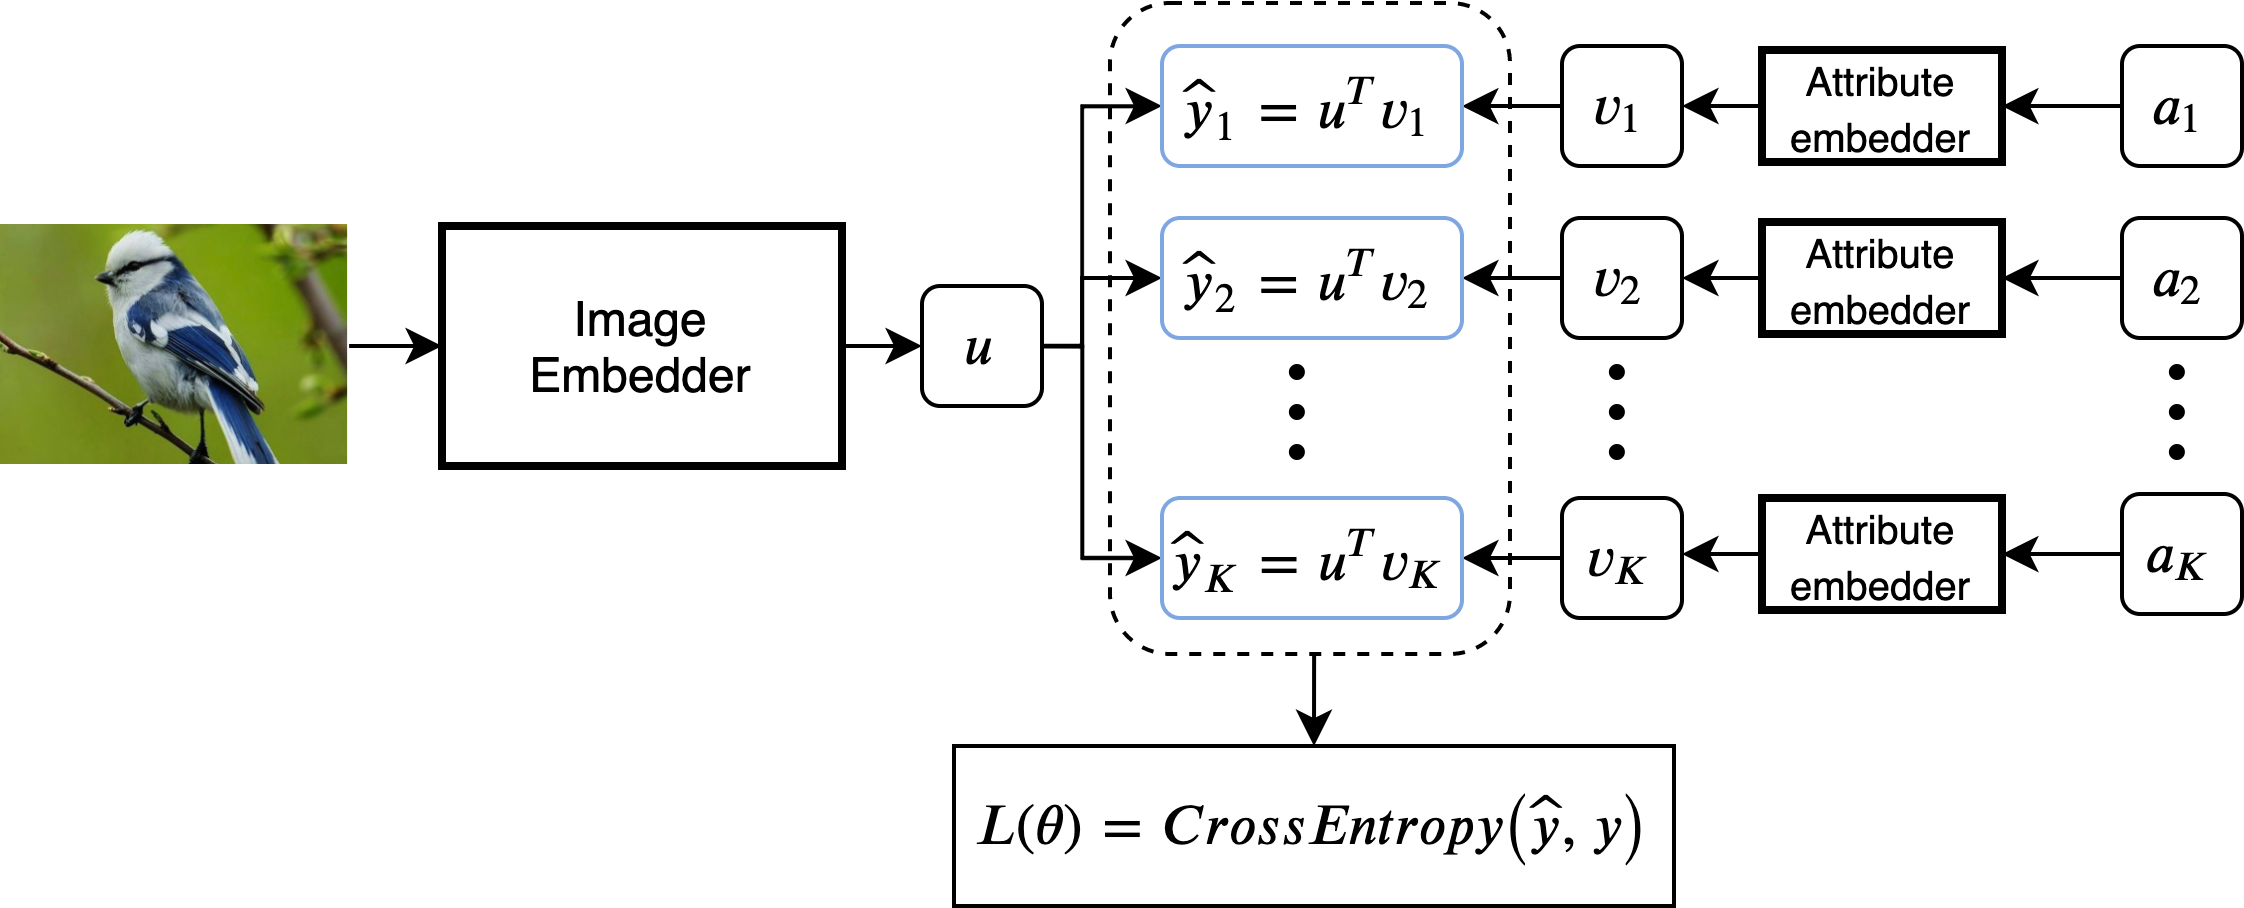
\includegraphics[width=\textwidth]{images/model-overview}
    \end{figure}
    
    \pause The approach is similar in spirit to metric learning:
    \begin{itemize}
        \item\pause Image embedder produces $u = f_\theta(x)$
        \item\pause Attribute embedder produces $v = g_\phi(a)$
        \item\pause We want the distance $d(u,v)$ to be low for proper pairs $x,a$ and large for improper ones.
    \end{itemize}
%    \begin{itemize}
%        \item We have image $X$, $K$ attributes $a_1, ..., a_K$ corresponding to $K$ classes and we want to tell to which of this attributes the image corresponds to.
%    \end{itemize}
\end{frame}


\begin{frame}{``Improved'' model}
Let's look closer at logits:

\begin{enumerate}
    \item\pause We compute $c$-th logit as $y_c = u^\top v_c$
    \item\pause (1) is very similar to $y_c = u^\top V_c u$ for diagonal matrix $V_c$ with $\text{diag}(V_c) = v_c$.
    \item\pause (2) is a special case of $(u - \mu_c)^\top V_c (u - \mu_c)$ (Maholonobis distance squared)
    \item\pause (3) is a part of gaussian log-density $\mathcal{N}(u|\mu_c, \Sigma_c)$
\end{enumerate}
\end{frame}


\begin{frame}{Building a generative model}
\begin{itemize}
    \item\pause So, let's define a generative model $p(u)$ as a GMM:
    \[
    p(u) = \sum_c \alpha_c \cdot \mathcal{N}(u | \mu_c, \Sigma_c)
    \]
    \item\pause Since our classes are balanced, we have $\alpha_c = P(y=c) = \frac{1}{K}$
    \item\pause Then, we can obtain $P(y_c | u)$ as:
    \[
    P(y_c | u) = \frac{p(u | y_c) P(y_c)}{p(u)} = \frac{\mathcal{N}(u | \mu_c, \Sigma_c) \cdot \frac{1}{K}}{\sum_c \frac{1}{K} \mathcal{N}(u | \mu_c, \Sigma_c)} = \frac{\mathcal{N}(u | \mu_c, \Sigma_c)}{\sum_c \mathcal{N}(u | \mu_c, \Sigma_c)}
    \]
    \item\pause This gives us a way to do log-likelihood maximization for $P(y_c|u)$
    \item\pause The only change is that we now compute logits as $\log \mathcal{N}(u | \mu_c, \Sigma_c)$:
    \[
    \log p(u|y_c) = \log \left[(2 \pi)^{-\frac{k}{2}} \operatorname{det}(\Sigma_c)^{-\frac{1}{2}} e^{-\frac{1}{2}(\mathbf{x}-\boldsymbol{\mu}_c)^{\top} \Sigma_c^{-1}(\mathbf{x}-\boldsymbol{\mu}_c)}\right]
    \]
\end{itemize}
\end{frame}


\begin{frame}{How to compute $\mu_c$ and $\Sigma_c$?}
\begin{itemize}
    \item\pause For attribute $a_c$ let's set $\mu_c = W_{\mu} a_c$ and $\Sigma_c = \mathbb{W}_{\Sigma} a_c$
    \item\pause But $\Sigma_c$ can be large, so $\mathbb{W}$ will be very expensive to use.
    \item\pause Solution: let's use low-rank + diagonal approximation for $\Sigma_c$:
    \[
    \Sigma_c = A\times B + \Lambda,
    \]
    where $A,B$ are low-rank matrices and $\Lambda$ is diagonal (to fix the rank).
    \item\pause A problem: in density computation for $\mathcal{N}(u | \mu_c, \Sigma_c)$ we need to compute $\det \Sigma_c$ and $\Sigma^{-1}_c$.
    \item\pause Solution: let's output $\Sigma^{-1}_c$ directly as $LL^{T}$ (Cholesky decomposition) and use the identity $\det \Sigma_c = 1/\det (\Sigma_c^{-1})$.
    \item\pause In clock-wall time, GMM vs baseline works 15\% slower on CUB and 0\% slower on AwA\footnote{Values taken from tqdm measurements on a single preliminary experiment}.
\end{itemize}
\end{frame}


\begin{frame}{Changes summary}
\pause
Old logit computation:
\[
\log p(u|y_c) = \log u^\top v_c
\]

\pause
New logit computation:
\[
\log p(u|y_c) = -\frac{1}{2} \log \det(\Sigma_c) -\frac{1}{2}(\mathbf{x}-\boldsymbol{\mu}_c)^{\top} \Sigma_c^{-1}(\mathbf{x}-\boldsymbol{\mu}_c)
\]

\pause
GMM differs from the baseline in 3 ways:
    \begin{enumerate}
        \item We use full-fletched covariance $\Sigma_c$: helps catching more entangled relationships
        \item We take into account the shift $\mu_c$
        \item We use determinant regularization for $\Sigma_c$
    \end{enumerate}

\pause
Additional benefit: we now have a principled generative model since our loss encourages discriminative training for $f(x)$ and generative training for $g(a)$ at the same time.
\end{frame}

\begin{frame}{Implementation details}
\pause
For each attribute $a_c$ predict 4 things:
    \begin{itemize}
        \item mean vector $\mu_c = W_\mu a_c$ of size $n$
        \item covariance diagonal $\sigma_c = W_\sigma a_c$ of size $n$
        \item covariance left matrix $A_c = \mathbb{W}_A a_c$ of size $n\times r$ (we set $r = 5$)
        \item covariance left matrix $B_c = \mathbb{W}_B a_c$ of size $r\times n$ (we set $r = 5$)
    \end{itemize}

\pause
Now we can compute inverse covariance:
\[
L_c^{-1} = \text{tril}(A_c \times B_c) + \text{Diag}(\sigma_c),
\]
where $\text{tril}(.)$ --- zeros out an upper triangle of a matrix and $\text{Diag}(.)$ --- constructs a diagonal matrix from a vector.

\pause
After that we compute 
\[
\Sigma^{-1} = (L_c^{-1})^\top L_c^{-1}
\]

\pause
Using $\mu_c$ and $\Sigma^{-1}$ we can now compute $\mathcal{N}(u | \mu_c, \Sigma_c)$ in a fast way.
    
\end{frame}


\begin{frame}{Experiments}

\begin{itemize}
    \item\pause Datasets
    \begin{itemize}
        \item CUB (200 classes): 20 tasks, 10 classes each
        \item AwA2 (50 classes): 10 tasks, 10 classes each
        \item NABirds (in progress)
    \end{itemize}
    \item\pause Only a single epoch per task, i.e. we see each example only once per lifetime
    \item\pause Hyperparameter search:
    \begin{itemize}
        \item Validation sequence: find the best hyperparams for a model on the first 3 tasks, then train the model on the rest with the best hyperparams.
        \item Use the same hyperparameters grid for both models
    \end{itemize}
    \item\pause Metrics: accuracy on seen, accuracy on unseen, harmonic mean, AUSUC, forgetting, etc.
\end{itemize}
\end{frame}

\begin{frame}{The problem}
The problem is that it does not quite work in practice...
\begin{itemize}
    \item Baseline model has normalize+scale trick which is \textit{crucial} to achieve good performance
    \item However, for the GMM this trick is not applicable
    \item How can we do normalize+scale for the GMM?
\end{itemize}
\end{frame}


\begin{frame}
    \frametitle{References}
    \printbibliography[heading=none]
\end{frame}
%\begin{frame}[noframenumbering,plain,allowframebreaks]{Literatur}
%    \printbibliography[heading=none]
%\end{frame}

\end{document}
